\documentclass{beamer}


\usepackage[T1]{fontenc}
\usepackage[utf8]{inputenc}
\usepackage{lmodern}
%\usepackage[a4paper,margin=0.85in]{geometry} % Réduire les marges
\usepackage[english]{babel}
\usepackage{amsmath}
\usepackage{amssymb}
\usepackage{amsthm}

\usepackage{cite} % Pour importer une bibliographie

\usepackage{bbm}
\usepackage{mathtools}
%\usepackage{ulem} % Pour barrer du texte
\usepackage{xcolor} % Pour colorer des symboles dans les équations


\DeclareMathOperator{\MAP}{MAP}

\title{Blind Deconvolution}
\date{January 9, 2018}
\author{Alexis THIBAULT}

\begin{document}
	
\begin{frame}{}
\maketitle
\end{frame}

\begin{frame}{Problem}
	Blurred image $y$
	\[
	y = k*x + w
	\]
	Unknown kernel $k$, noise $w$
	
	\uncover<2->
	{$\rightarrow$ Recover $x$ \emph{and} $k$}
	
	\begin{center}
	$y=$ \raisebox{-0.5\height}{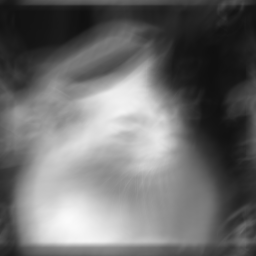
\includegraphics[width=2.5cm]{images/conv_louxor_large_kernel}}
	\uncover<3->
	{$\quad \xrightarrow{\quad ? \ldots} \quad$%
	$x=$ \raisebox{-0.5\height}{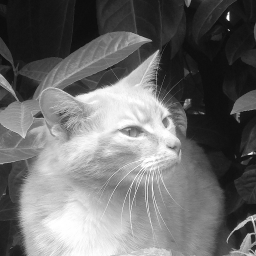
\includegraphics[width=2.5cm]{images/louxor}}
	, $k=$ \raisebox{-0.5\height}{
\includegraphics[width=1cm]{images/large_kernel}}
	}
	\end{center}
	
	\uncover<4->{More unknowns than equations $\rightarrow$ ill-posed.}
\end{frame}

\begin{frame}{Maximum a posteriori}
Strategy:
\begin{itemize}
	\item Initial probability density $p(x,k,y) = p(x)p(k)p(y\mid x,k)$
	\pause
	\item Find a `likely explanation' of $y$, by maximizing the \emph{a posteriori} probability
	\[
	(\MAP_{x,k}) \quad \quad (\hat{x},\hat{k}) = \arg \max p(x,k \mid y)
	\]
	\pause
	\item Alternative approach: find likely $k$, then deduce $x$.
	\[
	(\MAP_{k}) \quad \quad \hat{k} = \arg \max \int p(x,k \mid y) dx
	\]
\end{itemize}
\end{frame}
	
\begin{frame}{A priori distributions}
\begin{itemize}
	\item Natural images have (more or less) sparse derivatives
	\item Gaussian prior on the image: 
	\[
	p(x) \propto e^{-\frac{||\nabla x||_2^2}{\sigma^2}}
	\]
	\item Personal suggestion: Gaussian prior on the kernel
	\[
	p(k) \propto e^{-\frac{||\nabla k||_2^2}{\sigma_k^2}}
	\]
\end{itemize}
\end{frame}

\begin{frame}{Expectation-Maximization algorithm}
To compute $\MAP_{k}$, alternately update:
\begin{itemize}
	\item \[\mu,C := \text{ mean and covariance of } x \text{ given } (y,k)\]
	\item \[k := \arg \min E\left[||k*X - y||^2\right], \quad X\sim\text{Gaussian}(\mu,C) \]
\end{itemize}
\pause
Gaussian prior $\longrightarrow$ efficient computations in Fourier domain
\end{frame}

\begin{frame}{Results}
\centering
\raisebox{-0.5\height}{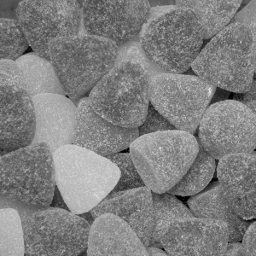
\includegraphics[width=2.5cm]{images/candy.png}}
\raisebox{-0.5\height}{$\;* $ }
\raisebox{-0.5\height}{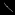
\includegraphics[width=0.5cm]{images/kernel3}}
\raisebox{-0.5\height}{$\;= $}
\raisebox{-0.5\height}{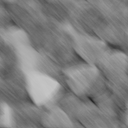
\includegraphics[width=2.5cm]{results/candy_kernel3_blurred.png}}
\\
\begin{tabular}{|l|l|l|}
	\hline
	$\MAP_{x,k}$ & $\MAP_{k}$ & $\MAP_{k}$ + kernel prior\\
	\hline
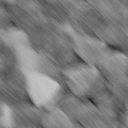
\includegraphics[width=2.5cm]{results/candy_kernel3_MAPxk_x.png}
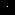
\includegraphics[width=0.5cm]{results/candy_kernel3_MAPxk_k.png}
&
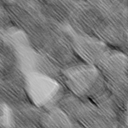
\includegraphics[width=2.5cm]{results/candy_kernel3_MAPk_x.png}
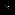
\includegraphics[width=0.5cm]{results/candy_kernel3_MAPk_k.png}
&
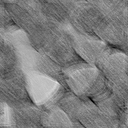
\includegraphics[width=2.5cm]{results/candy_kernel3_MAPkreg_x.png}
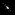
\includegraphics[width=0.5cm]{results/candy_kernel3_MAPkreg_k.png}
\\
\hline
\end{tabular}

\end{frame}
	

\begin{frame}{Conclusion}
\begin{itemize}
	\item $(\MAP_{x,k}) < (\MAP_{k}) \le (MAP_k$ + kernel prior$)$
	\pause
	\item Use better image prior:
	\begin{center}
		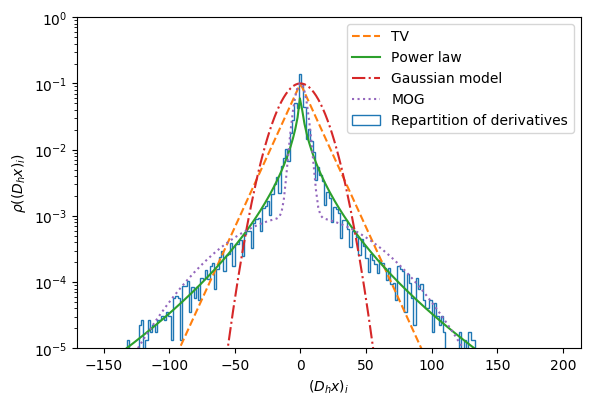
\includegraphics[width=7cm]{images/graph_derivatives}
	\end{center}
	\pause
	\item Better kernel priors?
\end{itemize}
\end{frame}

	
\end{document}